%
\section{The Fundamentals Behind SpatialDomains}
\label{sec:spatialdomains-fundamentals}

As mentioned in our discussions of the fundamentals of StdRegions (i.e. Section \ref{sec:stdregions-fundamentals}), one of the most
fundamental tools from calculus that we regularly employ is the idea of mapping from general domains to canonical domains.  General
domains are the regions in world space over which we want to solve engineering problems, and thus want to be able to take derivatives and
compute integrals.  But as we learned in calculus, it is often non-trivial to accomplish differentiation or integration over these regions.  We resort
to the mapping arbitrary domains back to canonical domains over which we can define various operations.  We introduced our canonical domains,
which we call standard regions, in Chapter \ref{chap:stdregions}.  We refer to our world space regions as local regions, which we will present
in Chapter \ref{chap:localregions}.  How these two are connected are via SpatialDomains.  

As will be further discussed in Section \ref{sec:spatialdomains-datastructures}, there are two fundamental purposes served by SpatialDomains:  (1) holding
basic geometric information (e.g. vertex values and curvature information) and (2) holding geometric factors information.  The former information relates to 
the geometric way we map standard regions to local regions.  The latter information relates to how we use this map to allow us to accomplish 
differentiation and integration of functions in world space via operations on standard regions with associated map (geometric) information.  In this section,
we will highlight the important mathematical principles that are relevant to this section. We will first discuss the mapping itself:  vertex and curvature information
and how it is used.  We will then discuss how geometric factor information is computed.  We break this down into two subsections following the convention of the
code.  We will first discussed what is labeled in the code as {\em Regular}, and denotes mappings between elements of the same dimension 
(i.e. standard region triangles to 2D triangles in world space).  Although our notation will be slightly different, we will use \cite{KaSh05} as our guide; we
refer the interested reader there for a more in-depth discussion of these topics. 
We will then discuss what is labeled in the code as {\em Deformed}, and denotes the mappings 
between standard region elements and their world space variants in a higher embedded dimension (i.e. standard region triangles to triangles lying on a 
surface embedded in a 3D space representing a manifold).  Since the manifold work within {\nek} was introduced as an area of research, we will
use \cite{CantwellYKPS14} as our guide.  The notation therein is slightly different than that of \cite{KaSh05} because of the necessity to use
broader coordinate system transformation principles (e.g. covariance and contravariance of vectors, etc.).   We will abbreviate the detailed
mathematical derivations here, but encourage the interested reader to review \cite{CantwellYKPS14} and references therein as needed.  For those
unfamiliar with covariant and contravariant spaces, we encourage the reader to review \cite{BorisenkoTS}.

\subsection{Vertex and Curvature Mapping Information}

When we load in a mesh into {\nek}, elements are often described in world space based upon their vertex positions.  In traditional FEM formats, this can be as
simple as a list of d-dimensional vertex coordinates, followed by a list of element definitions:  each row holding four integers (in the case of tetrahedra) denoting
the four vertices in the vertex list that comprise an element.   {\nek} uses an HTML-based geometry file with a more rich definition of the basic geometric
information that just described; we encourage developers and users to review our User Guide(s) for the organization and conventions used within our geometry 
files.  For the purposes of this section, the important pieces of information are as follows.  Let us assume that for each element, we have through our MeshGraph
data structure (described in the next section) access to the vertex positions of an element.   In general, each vertex $\vec{v}_j$ is a n-tuple of dimension $d$ denoting
the dimension in which the points are specified in world space.  For example, when considering a quadrilateral on the 2D plane, our vertex points each contain
two coordinates denotes the x-- and y--coordinates.  As shown in Figure \ref{spatialdomains:planarmap}, we can express the mapping between a world space
quadrilateral and the standard region quadrilateral on $[-1,1]\times[-1,1]$ via a bi-linear mapping function $\chi(\vec{\xi})$.

\begin{figure}[htb]
\centering
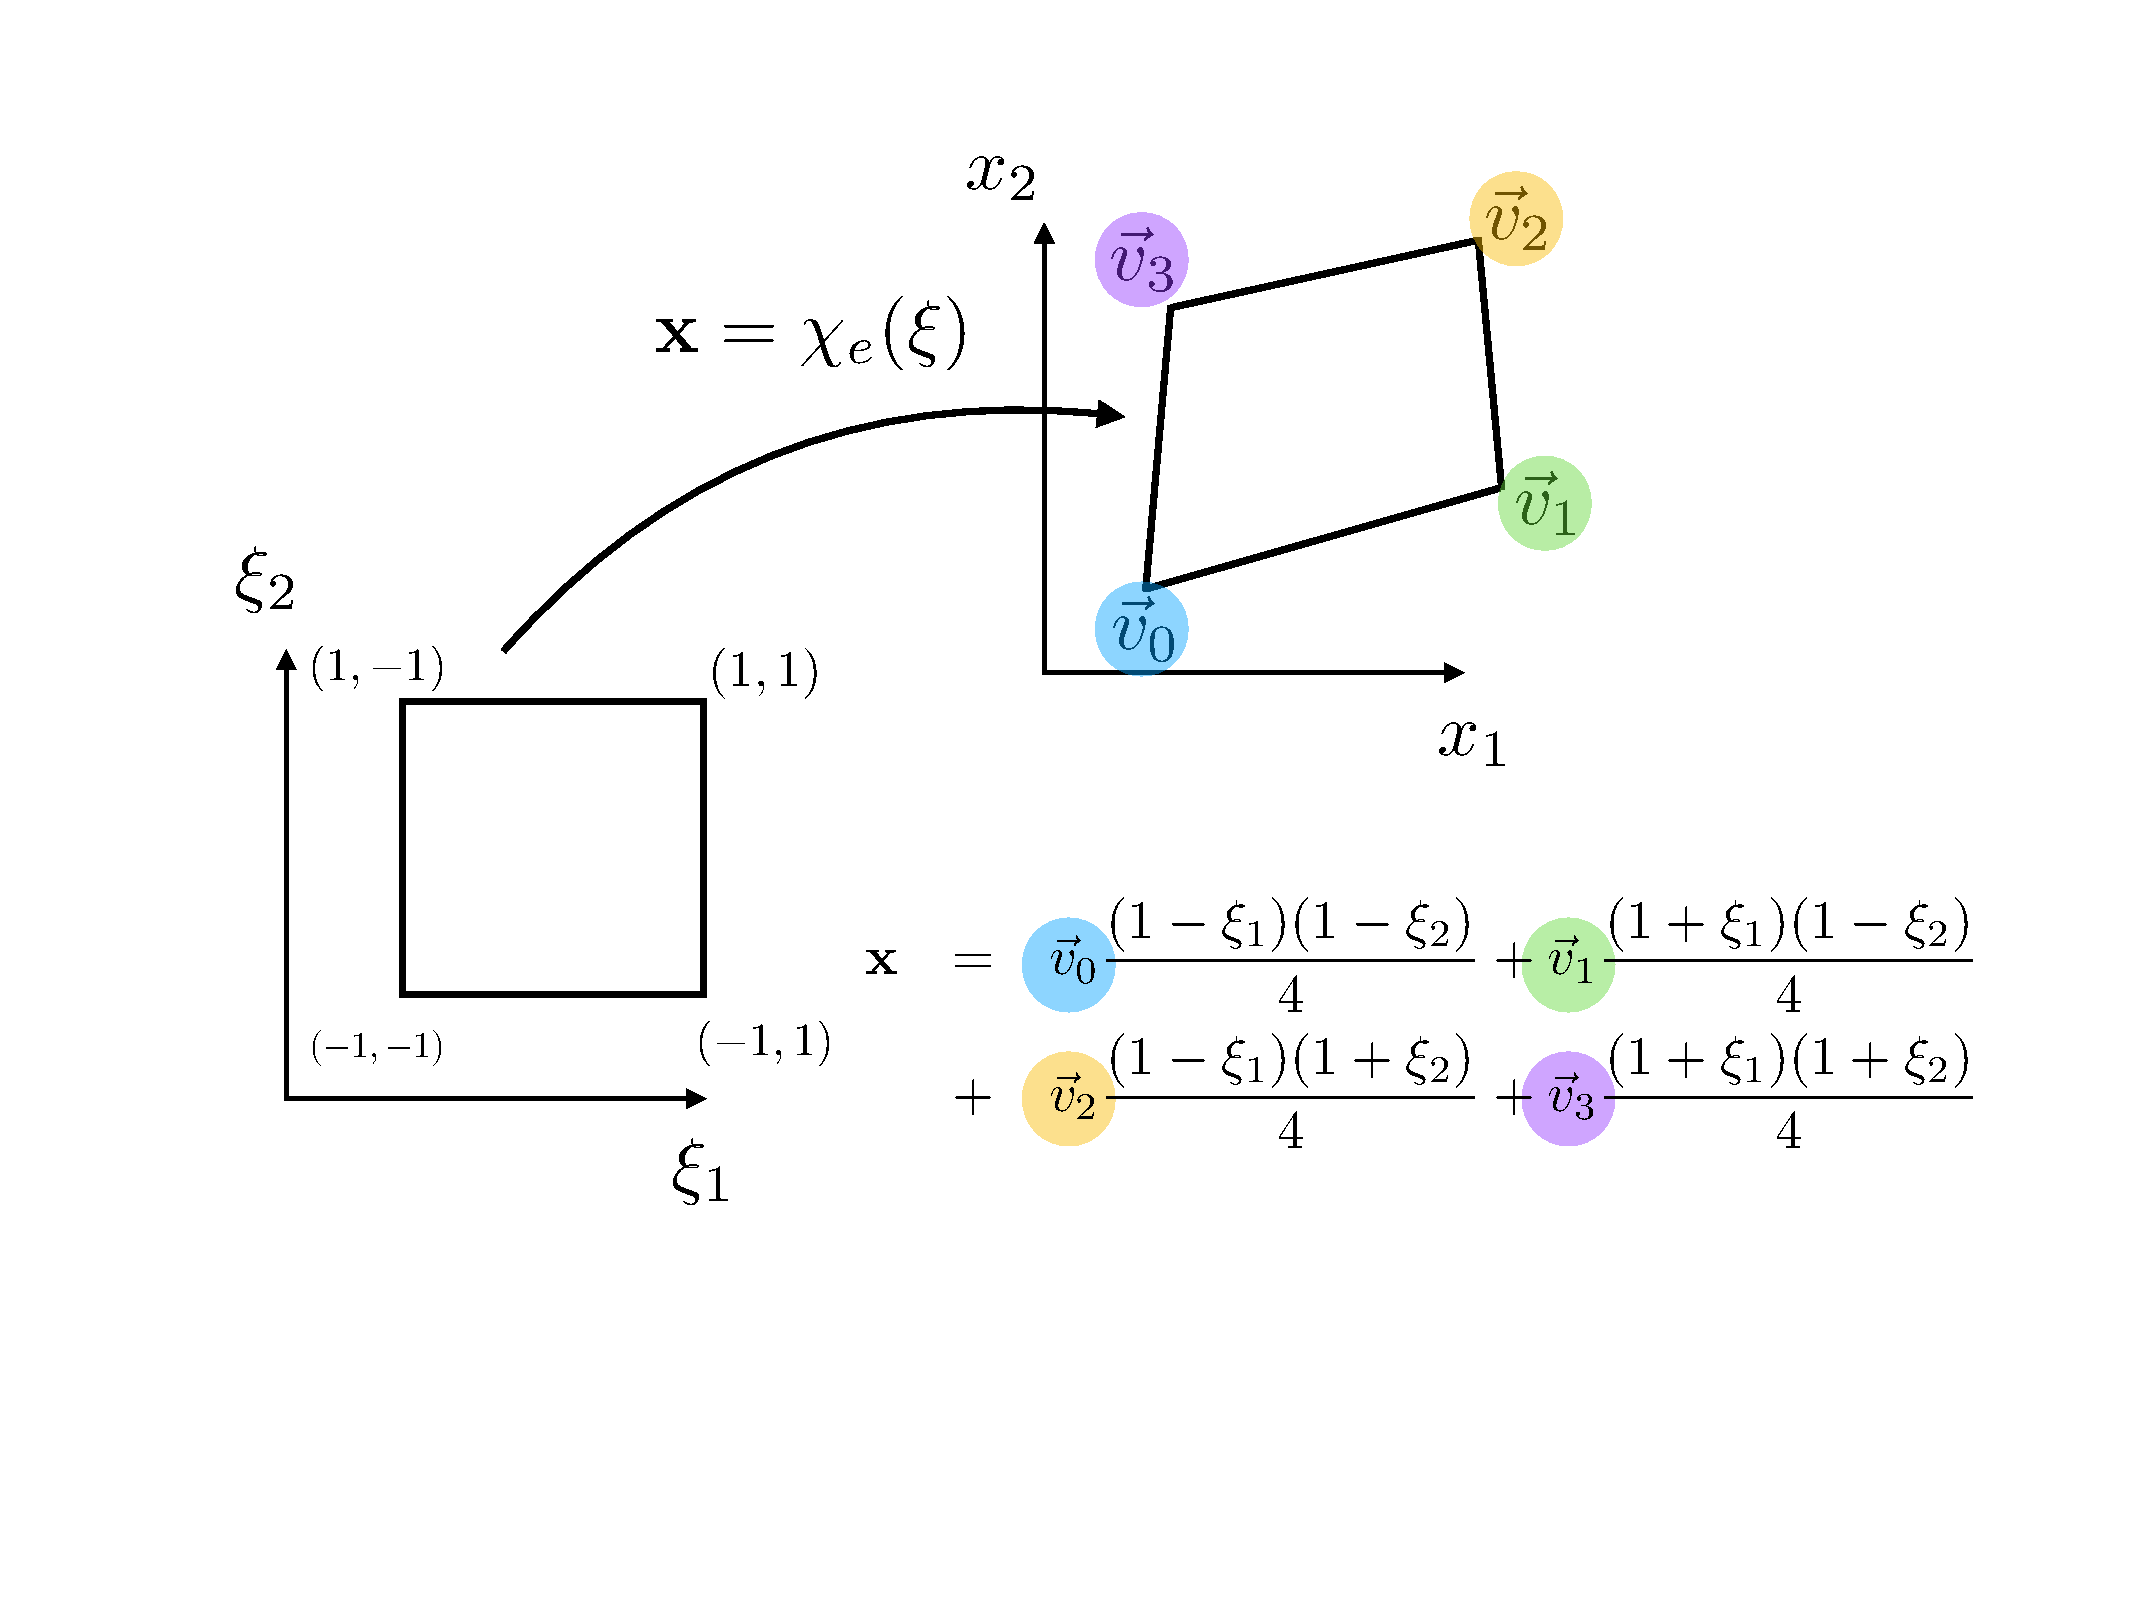
\includegraphics[width=6in]{img/planarmap.pdf}
\caption{Reference space to world space mapping of a 2D quadrilateral to a straight-sided (2D) quadrilateral in the plane via a bi-linear (i.e., $Q(1)$) mapping.}
\label{spatialdomains:planarmap}
\end{figure}

In the case of segments, this mapping function $\chi(\vec{\xi})$ is a function of one variable and is merely an affine mapping.  In two dimensions, the 
mapping of a straight-sided triangle is a linear mapping (i.e., P(1) in the language of traditional finite elements -- a total degree $k=1$ space) and
the mapping of a straight-sided quadrilateral is a bi-linear mapping (i.e, Q(1) in the language of traditional finite elements -- a degree $k=1$ map along each
coordinate direction combined through tensor-product).  In three dimensions, the mapping of a planar-sided tetrahedron is also a linear mapping, the
mapping of a planar-sided hexahedron is a tri-linear mapping, and the prism and pyramid are mathematically somewhere in-between these two canonical
types as given in \cite{KaSh05}.  The key point is that in the case of straight-sided (or planar-sided) elements, the mapping between reference space and
world space can be deduced solely based upon the vertex positions.  Furthermore in these cases, 
as denoted in Figure \ref{spatialdomains:planarmap}, the form of the mapping function is solely determined by type (shape) of the element.  If
only planar-sided elements are used, pre-computation involving the mapping functions can be done so that when vertex value information is available,
all the data structures can be finalized.  

As presented in \ref{KaSh05}, there are many components of {\nek} that capitalize on the geometric nature of the basis functions we use.  We often
speak in terms of vertex modes, edge modes, face modes and internal modes -- i.e., the coefficients that provide the weighting of vertex basis functions,
edge basis functions, etc.  It is beyond the scope of this developer guide to go into all the mathematical details of their definitions, etc.  However, we do 
want to point out a few common developer-level features that are important.   In the case of straight-sided (planar-sided) elements, the aforementioned
mapping functions can be fully described by vertex basis functions.  The real benefit of this approach (of connecting the mapping representation with a
geometric basis) is seen when moving to curved elements.

Consider Figure \ref{spatialdomains:curvemap} in which we modify the example given above to accommodate on curved edge.  From the 
mathematical perspective, we know that the inclusion of this (quadratic) edge will require our mapping function to now be in $Q(2)$.  If we were
not to use the fact that our basis is geometric in nature, we would be forced to form a Vandermonde system for a set of coefficients used
to combine the tensor-product quadratic functions (nine basis functions in all), and use the five pieces of information available to us (the four
vertex values and the one point $\vec{c}_0$ that informs the curve on edge $1$.   As shown in Figure \ref{spatialdomains:curvemap}, we would
expect that this updated (to accommodate a curved edge) mapping function to consist of the bi-linear mapping 
function with an additional term $C_1(\xi_1,\xi_2)$ that encompasses the new curvature information.  

\begin{figure}[htb]
\centering
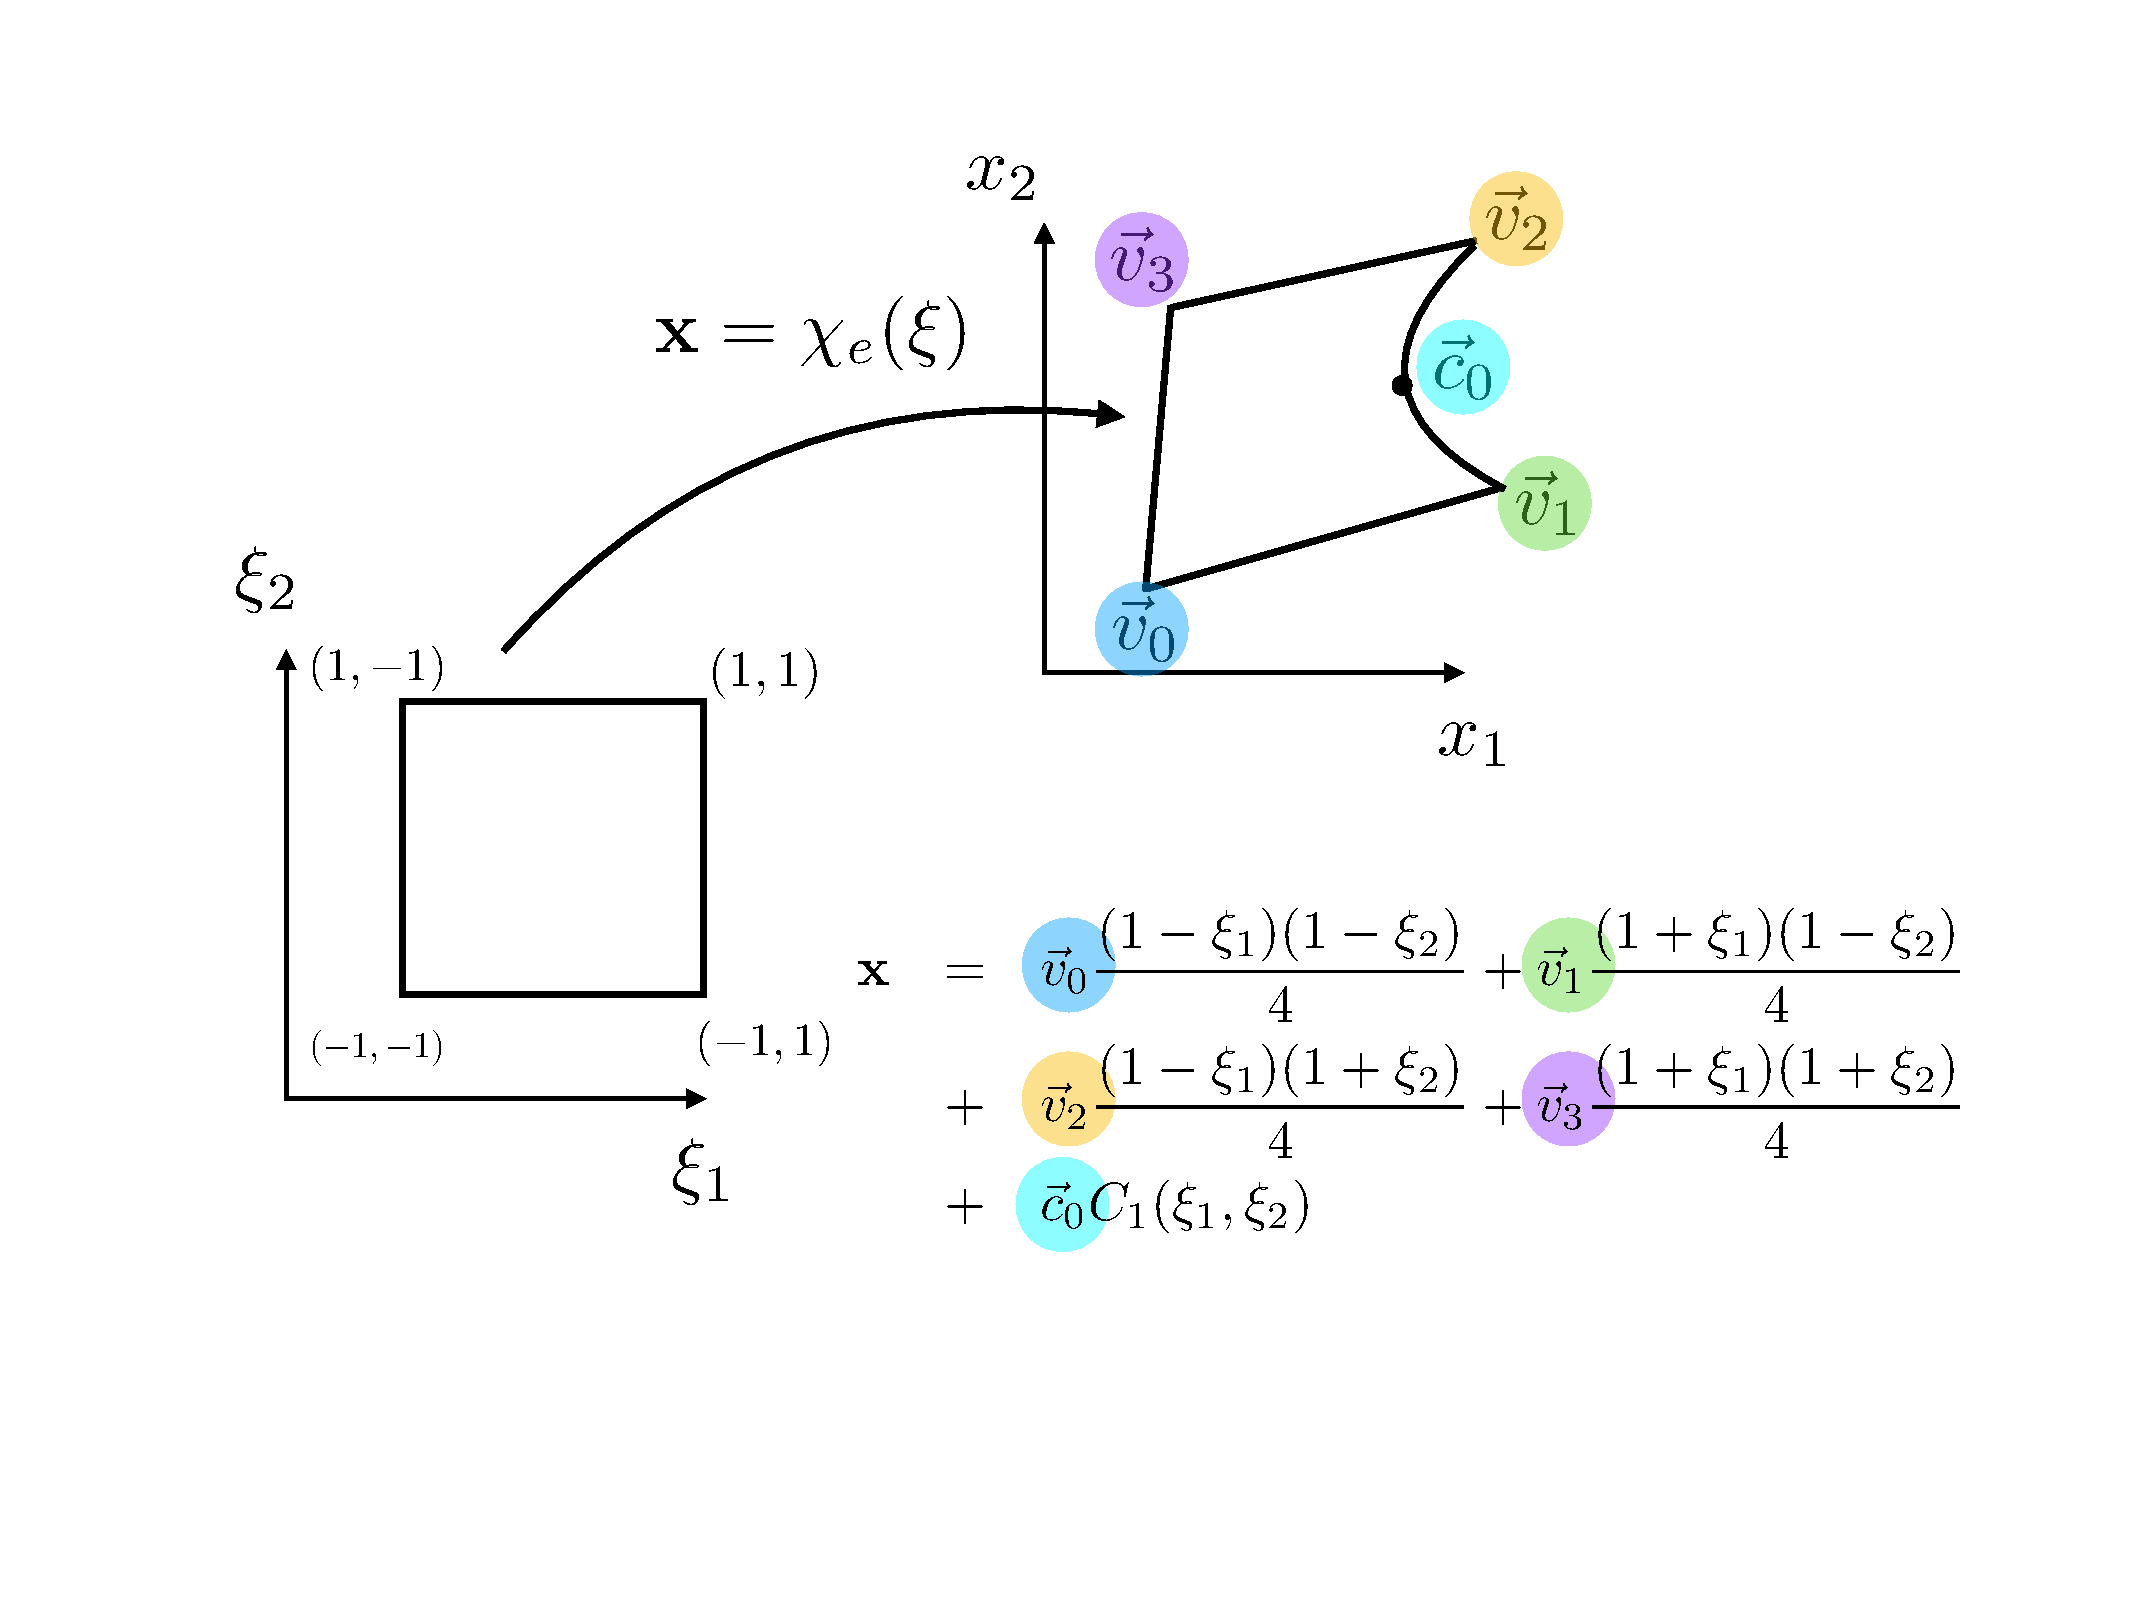
\includegraphics[width=6in]{img/curvemap.pdf}
\caption{Reference space to world space mapping of a 2D quadrilateral to a curve (2D) quadrilateral in the plane via a bi-quadratic (i.e., $Q(2)$) mapping.}
\label{spatialdomains:curvemap}
\end{figure}

The basis we use, following \cite{KaSh05}, allows us to precisely specify $C_1(\xi_1,\xi_2)$ using the edge basis function associated with edge $1$, and
to use the point value $\vec{c}_0$ to specify the coefficient to be used.  In the figure, we assume that the form of the function is collocating, but in practice
it need not be so.  

In practice, edge (and face) information can be given either as a set of point positions in world space that correspond to a particular point distribution 
in the reference element (i.e., evenly-spaced points or GLL points) or modal information corresponding to the geometric basis we use internally.  Our
geometric file formats assume the former -- that curve information is provided to us as physical values at specified positions from which we infer (calculate)
the modal values and store these values within SpatialDomain data structures.

Assuming we now have, for each element, a way of specifying the mapping function $\chi(\vec{\xi})$, we can now move to how we compute the geometric 
factors for regular as well as for deformed mappings. 
We use the term ``regular mappings" to refer to mappings from reference space elements to world space elements with the same dimension.  For instance, a 
collection of triangles that lie in a plane can be represented by vertex coordinates that an only 2-tuples and the mappings between the reference space
triangle the and world space triangle does not need to consider a larger embedded dimension.  This was a fundamental assumption of the original
Nektar code:  segments lived on the 1D line, triangles and quadrilaterals lived on the 2D plane and that hexahedra, tetrahedra, etc., lived in the 3D 
volume.   When redesigning {\nek}, we purposefully enabled geometric entities to live in a high-dimensional embedding space, different from their
parameterized dimension.  For instance, in {\nek}, it is possible to define segment expansions (functions that live over one dimensional parameterized
curves) that are embedded in 3D.  The same is true for quadrilaterals and triangles -- although their parameterized dimension is two, both may live in
a higher dimensional embedding space and thus represent a {\em manifold} of co-dimension one in that space.  For mappings that maintain the
co-dimension is the opposite of the dimension (i.e., quadrilateral in a plane represented by vertices with two coordinates mapped to a two parameter 
reference quadrilateral), we keep to the mapping conventions originally outlined in \cite{KaSh05} and denote these mapping operations in the code by the enumerated 
value {\em Regular}; for mappings in which the co-dimension is greater than zero, we following the modified convention outlined in \cite{CantwellYKPS14} and denote
these mapping operations in the code by the enumerated value {\em Deformed}.

\subsection{Regular Mappings: Geometric Factors}

Following \cite{KaSh05}, we assume that the vertex positions of an element in world space are given by $\vec{x} = x_i$ and that our reference space
coordinates are given by $\vec{\xi} = \xi_j$, there $i \text{ and } j$ run from zero to $dim-1$ where $dim$ is the parameter dimension of the element (e.g.
for a triangle, $dim = 2$).

The Jacobian (matrix) is correspondingly defined as:

\begin{equation} \label{eqn:jacobianmat}
{\bf J} = \frac{\partial x_i}{\partial \xi_j}.
\end{equation}

Note that this matrix is always square, but also note that it is not always constant across an element.  Only in special cases such as the 
linear mapping of triangles and tetrahedra does the Jacobian matrix reduce to a constant (matrix) over the entire element.  In general, 
this matrix can be evaluated at any point over the element for which it is constructed.

There are two (high-level) times in which this information is needed: when computing derivatives and when computing
integrals.  When computing derivatives, we employ the chain rule for differentiation, which in Einstein notation is given by the following expression:

$$
\frac{\partial}{\partial x_i} = \frac{\partial \xi_j}{\partial x_i} \frac{\partial}{\partial \xi_j}.
$$

Note that this expression requires the reciprocal of the expression above -- that is, ${\bf J}^{-1}$.  The polynomial mappings we use in {\nek}
are defined in terms of their forward mappings (reference to world).  If the determinant of the mapping is non-zero, the inverse of the mapping
exists but is not available analytically (except is special cases).  As a consequence, we in general limit the places at which we compute
the inverse of the Jacobian.  Typically, the quadrature point positions are the places at which you need these values (since it as at these
points we take physical space derivates and then use integration rules to construct weak form operators).  Thus, procedurally, we do the following:

\begin{enumerate}
\item For a given element, compute the Jacobian matrix using the expression given in Equation \ref{eqn:jacobianmat} for each quadrature point
position on the element (or for any points positions within an element at which it is needed).
\item Explicitly form the inverse of the matrix at each point position.
\end{enumerate}

Because we accomplish the inversion of the Jacobian matrix at particular positions, this introduces an approximation to this computation.
Although the inverse Jacobian matrix can be computed exactly at each point -- when we then correspondingly use this information 
in the inner product over an element -- we are in effect assuming that we are using a polynomial interpolative projection of this operator.
The approximation error is introduced at the point of our quadrature approximation.  Although the forward mapping is polynomial and hence
we could find a polynomial integration rule and number of points/weights to integrate our bilinear forms exactly, our use of the inverse
mapping in our bilinear forms means that we can only approximate our integrals.  From our experiments, the impact of his is negligible
in most cases, and only becomes in a concern in highly curved geometries.  In such cases, over-integration might be requires to minimize
the errors introduced due this approximation.

The other place at which we need the Jacobian matrix is to compute its determinant to be used in integration.  The determinant of the Jacobian
matrix (sometimes also called ``the Jacobian" of the mapping) provides us the scaling of the metric terms used in integration.  In all our
computations, we assume that the determinant of the Jacobian matrix is strictly positive.   In the area of mesh generation, the value 
of the determinant is used to estimate how good or bad the quality of the mapping is -- in effect, if you have reasonable elements in your mesh.
Negative Jacobian elements are inadmissible but even elements with small Jacobian determinants might cause issues.   At
the level of the library and solvers, we assume that these issues have been addressed by the user prior to attempting to run {\nek}
solvers and interpret their results.


\subsection{Deformed Mappings: Geometric Factors}

Following \cite{CantwellYKPS14}, we again assume that the vertex positions of an element in world space are given by $\vec{x} = x_i$ and that our reference space
coordinates are given by $\vec{\xi} = \xi_j$, there $i$ runs from zero to $dim-1$ where $dim$ is the embedding dimension and $j$ runs from zero to $M-1$ where $M$
is the parameter dimension of the element (e.g.for a triangle on a manifold embedded in 3D with vertex values in 3D, $dim = 3$ whilst $M=2$).

The Jacobian (matrix) is correspondingly defined as:

\begin{equation} \label{eqn:jacobianmat}
{\bf J} = J^i_j = \frac{\partial x_i}{\partial \xi_j}.
\end{equation}

In this case, we use the notational conventions of \cite{Ar89} which delineate covariant and contravariant forms. In general, this matrix is not square, 
also also note that it is not always constant across an element.  In general, this matrix can be evaluated at any point over the element for which it is constructed.
The metric tensor related to this transformation can be formed as:

$$
{\bf g} = {\bf J}{\bf J}^T
$$

\noindent and the Jacobian factor associated with this mapping is then given by:

$$
g = \det{\bf g}.
$$

Because various mappings are necessary when dealing with covariant and contravariant vectors, we have encapsulated all these routines 
into the directory GlobalMapping (see Chapter \ref{chapter:globalmapping}).  At this stage, we do not implement general Piola transformations \cite{McRaeBMHC} that further respect $H(div)$ and $H(curl)$ constraints on these mappings
as would be needed in solid mechanics or electromagnetics; however, there is nothing inherent within the {\nek} framework that would preclude someone from
adding these additional features as necessary.


